%%%%%%%%%%%%%%%%%%%%%%%%%%%%%%%%%%%%%%%%%%%%%%%%%%%%%%%%%%%%%%%%%%%%%%%%%%%%%%%%
%2345678901234567890123456789012345678901234567890123456789012345678901234567890
%        1         2         3         4         5         6         7         8

\documentclass[letterpaper, 10 pt, conference]{ieeeconf}  % Comment this line out if you need a4paper

%\documentclass[a4paper, 10pt, conference]{ieeeconf}      % Use this line for a4 paper

\IEEEoverridecommandlockouts                              % This command is only needed if
                                                          % you want to use the \thanks command

\overrideIEEEmargins                                      % Needed to meet printer requirements.

%In case you encounter the following error:
%Error 1010 The PDF file may be corrupt (unable to open PDF file) OR
%Error 1000 An error occurred while parsing a contents stream. Unable to analyze the PDF file.
%This is a known problem with pdfLaTeX conversion filter. The file cannot be opened with acrobat reader
%Please use one of the alternatives below to circumvent this error by uncommenting one or the other
%\pdfobjcompresslevel=0
%\pdfminorversion=4

% See the \addtolength command later in the file to balance the column lengths
% on the last page of the document

% The following packages can be found on http:\\www.ctan.org
%\usepackage{graphicx}
%\usepackage{graphics} % for pdf, bitmapped graphics files
%\usepackage{epsfig} % for postscript graphics files
\usepackage{mathptmx} % assumes new font selection scheme installed
%\usepackage{times} % assumes new font selection scheme installed
\usepackage{amsmath} % assumes amsmath package installed
\usepackage{amssymb}  % assumes amsmath package installed
\newcommand{\transpose}[1]{\ensuremath{#1^{\scriptscriptstyle T}}}
% --------------- GRAPHIC PACKAGES ----------------------------
\usepackage{graphicx}
\graphicspath{{./images/}}
\usepackage{xcolor}



% --------------- Document Info ----------------------------

\title{\LARGE \bf Quaternion EKF }

\author{Albert Author$^{1}$ and Bernard D. Researcher$^{2}$% <-this % stops a space
\thanks{*This work was not supported by any organization}% <-this % stops a space
\thanks{$^{1}$Albert Author is with Faculty of Electrical Engineering, Mathematics and Computer Science,
        University of Twente, 7500 AE Enschede, The Netherlands
        {\tt\small albert.author@papercept.net}}%
\thanks{$^{2}$Bernard D. Researcheris with the Department of Electrical Engineering, Wright State University,
        Dayton, OH 45435, USA
        {\tt\small b.d.researcher@ieee.org}}%
}


\begin{document}



\maketitle
\thispagestyle{empty}
\pagestyle{empty}


%%%%%%%%%%%%%%%%%%%%%%%%%%%%%%%%%%%%%%%%%%%%%%%%%%%%%%%%%%%%%%%%%%%%%%%%%%%%%%%%
\begin{abstract}

Pose estimation has long been a subject of interest to researchers\\

This paper presents an EKF based pose estimation and tracking for situations where direct sensing is not feasible. We expand on the work of Fathian and Dani, \cite{quest} and \cite{vest}, by using their vision based pose and velocity estimation as remote sensing measurements to our EKF model.


Short sentences on what we will present

\end{abstract}


%%%%%%%%%%%%%%%%%%%%%%%%%%%%%%%%%%%%%%%%%%%%%%%%%%%%%%%%%%%%%%%%%%%%%%%%%%%%%%%%
\section{INTRODUCTION}

\textbf{Similar to Abstract but in past tense and in more detail}\\

In this paper, we combine QUEST and VEST with Kalman Filter.\\

\subsection{Background}

% start with the template for structure and how the material is presented!!
The Kalman Filter (KF) was formally introduced in the summer of 1960 by Rudolf E. Kalman where, he formulated the state-space representation of dynamical systems \cite{KF}.




\subsection{Notation}
% For clarity, we dedicated this section to formally present the notation used in this paper.
Vectors are represented by normal font variables, i.e. $a,x,y,z$.
Matrices are represented by UPPERCASE letters, i.e. $\mathbf{A,X,Y,Z}$.
\textit{Approximation} vectors are denoted with a \textit{tilde} i.e. $\widetilde{a},\widetilde{x},\widetilde{y},\widetilde{z}$.
We define approximate function representation
in \ref{eq:3} and \ref{eq:4} as the original function with added bias and uniform distribution noise.
This form of representation is used to express measurements that
are used as approximate control input to the system. This is an essential part the EKF
implementation, which we describe in detail in later sections.
\textit{Estimation} vectors are represented with a \textit{hat}, i.e. \(\widehat{a},\widehat{x},\widehat{Y},\widehat{Z}\).


\subsection{Paper Structure}


\section{OBSERVATION AND ESTIMATION MODELS}

\subsection{Inertial Model}

We start with a basic linear continuous-time state-space representation of a dynamical system and derive


For this paper, we used linear and angular velocities obtained from  as known input
to the system, where we define $u \in \mathbb{R}^6$ as,

\begin{equation} \label{eq:1}
\transpose{u} := \left[ \transpose{v} \transpose{\omega} \right],
\end{equation}

\begin{equation} \label{eq:2}
u_{B} =
\begin{bmatrix}
        {C}^{I}_{B}  \\
        {C}^{I}_{B}  \\
\end{bmatrix} u,
\end{equation}

\noindent
where matrix ${C}^{I}_{B}$ represents the orthanormal rotation from \textit{inertial frame},
\textit{I}, to robots \textit{body frame}, \textit{B}.



\begin{equation} \label{eq:3}
\widetilde{v}= v + n_{v} + b_{v},
\end{equation}


\begin{equation} \label{eq:4}
\widetilde{\omega} = \omega + n_{\omega} + b_{\omega}.
\end{equation}

\noindent
where $n$ and $b$ represent a uniform distribution or Brownian noise and bias from the measurement. Both $n$ and $b$ belong to $\mathbb{R}^3$


\subsection{Linearization}


\subsection{Discretization}

\subsection{QUEST}


\subsection{VEST}



\subsection{Observation State Definition}

The measurement state definition is defined by linear position, $r$, linear
velocity, $v$, angular velocity, $\omega$, and angular orientation in the quaternion
space, $q$. The observation state vector, $z$, is defined as the following:

\begin{equation} \label{eq:5}
\transpose{z} :=  \left[\transpose{r}~\transpose{v}~\transpose{\omega}~\transpose{q_{xyzw}} \right],
\end{equation}


Where the observed the quaternion state is used to compute the corresponding state
rotation matrix, ${C}^{I}_{B}$.
It is important to note that the observation data for position and orientation are treated as \textit{estimation groundtruth} (Keep?????) and velocity values are treated as \textit{control inputs} to the system. Both estimation groundtruth and control inputs carry \textit{process and observation noise}, respectively.




\subsection{EKF Model}

We deployed a modified EKF filter that uses \textit{Quaternion} for representing
rotations. We explain these modifications in detail in the \textit{Quaternion Algebra}.
We start with a nonlinear continuous-time system model described by,

\begin{equation} \label{eq:6}
\dot{x} = f(x,u),
\end{equation}
\begin{equation} \label{eq:7}
y = h(x,u).
\end{equation}

Where $f()$ represents the \textit{process} model and $h()$ represent the
\textit{observation} model.
Variables $\omega_{f}$ and $\omega_{h}$ represent the \textit{process} and \textit{observation} noise, respectively.
Vector $u$ represents input to the system and $u \in \mathbb{R}^{6}$ .
Vector $y$ represents the system output and $y \sim \in \mathbb{R}^6$ .





\section{QUATERNION ALGEBRA} \label{sec:QuatAlg}

Quaternion space is a non-minimal representation belonging to \textit{SO(3)} Lie group.

\subsection{Unit Quaternion}
Moreover, the quaternion term from the dataset has \textit{four terms} with $xyzw$
format.
Hamilton's quaternion defined by 3 perpendicular imaginary axes $i,j,k$ with
real scalars $x,y,z$ and a real term $w$, which constraints other 3 dimension to
a \textit{unit magnitude}. Thus, the fourth term normalizes the vector's magnitude
conveniently and preserves the 3D rotation (3 DOF). We define \textbf{Unit Hamiltonian}
or \textbf{Unit Quaternion} as,


\begin{eqnarray}\nonumber
\label{eq:9}
\mathbb{H}^{1} &:=&\left\{ q_{wxyz}=w+xi+yj+zk~\in \mathbb{H}~| \right.\\
                   && \left.~w^{2}+x^{2}+y^{2}+z^{2}=1 \right\}
\end{eqnarray}
% page 27, sec 2.4.2 of "Quaternion Algebra"
\noindent
where superscript 1 in $\mathbb{H}^{1}$ denotes a unit quaternion space with 4
terms. There are two equal representations for $\mathbb{H}^{1}$ subgroup; thus,
we provide a concise definition and notation for both to avoid confusion. The
the first representation is shown in \ref{eq:5} where the four terms of the
quaternion are arranged in $wxyz$ order and it is represented by $q_{wxyz}$.
The second quaternion is arranged in $xyzw$ format and is represented by $q_{xyzw}$.
It is important to note the difference as both are used in our derivation and
implementation.

\begin{equation}
\label{eq:12}
q_{wxyz} = q_{xyzw} ~; ~~~ q_{wxyz},~q_{xyzw} \in \mathbb{H}^{1}
\end{equation}


\subsection{Pure Quaternion}
As previously mentioned, the three imaginary terms of the quaternion represent the
3D angles of interest in radians and the fourth dimension constraints the vector
magnitude. Thus to avoid computational errors, in the prediction step, we use
the unit quaternion where it only has its three imaginary terms, $xyz$.
This quaternion space representation is defined by $\mathbb{H}^{0}$ and
denoted by $q_xyz$ variables.



\begin{eqnarray}\nonumber
\label{eq:13}
\mathbb{H}^{0} &:=& \left\{ q_{xyz}=xi+yj+zk~ \in \mathbb{H}~| \right.\\
&& \left. ~x,y,z \in \mathbb{R} \right\} \backsimeq  \mathbb{R}^3
\end{eqnarray}
% page 27, sec 2.4.2 of "Quaternion Algebra"



\subsection{Exponential Map}

For calculating incremental rotation in

Incremental rotation estimation using the skew-symmetric matrix obtained form
the rotational rate vector and matrix exponential mapping function, [QEKF01].
Gamma, $\Gamma$, represents incremental

\begin{equation}
\label{eq:14}
\Gamma_{0} := \sum_{i=0}^{\infty} \frac{ \left( \Delta t^{i+n}  \right)}{ \\
\left( i + n \right) \! } \\
\omega^{\times i},
\end{equation}

Where $(.)^{\times}$ represents skew-symmetry matrix of a vector


\subsection{Updating Quaternion State}
\begin{equation}
\label{eq:15}
q_{i+1} = \delta q_{i} \otimes \widehat{q}_{i}
\end{equation}



\subsection{Capturing Quaternion Error}
We use the mapping function $\zeta(.)$ to calculate the quaternion
state error from the error rotation vector, [QEKF01].

\begin{equation}
\label{eq:16}
\delta q = \zeta(\delta \phi),
\end{equation}

\begin{equation}
\label{eq:17}
\zeta : v \rightarrow \zeta(v) =
        \begin{bmatrix}
        \sin(\frac{1}{2}\|v\|) \frac{v}{\|v\|} \\
        \cos(\frac{1}{2}\|v\|)
        \end{bmatrix}
\end{equation}

\section{System Modeling and Linearization}

\subsection{Nonlinear Discrete Model}
% # eq 16-22 of QEKF2
The QEKF2 paper (State Estimation for a Humanoid Robot) has the following discrete
nonlinear model.

\begin{figure}[h]
  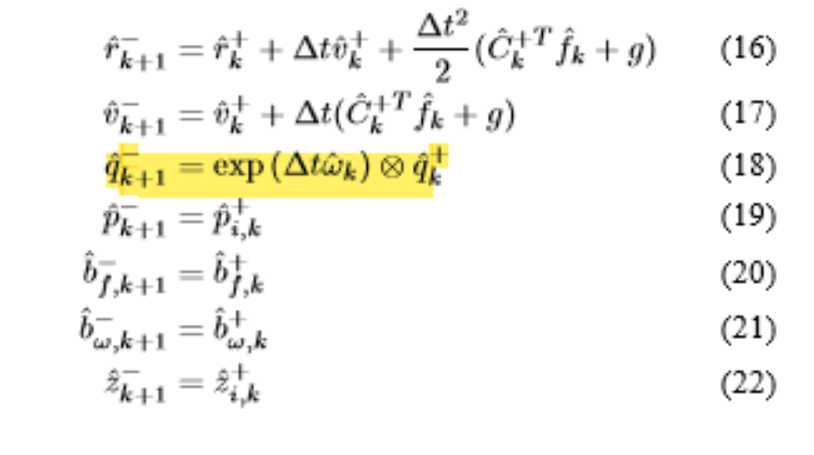
\includegraphics[width=.45\textwidth]{fig01.png}
  \centering
\end{figure}




\section{Extended Kalman Filter}
The Kalman Filter algorithm is capable of handling minor nonlinearities due to measurement
noise by forming approximate Gaussian distributions about the state estimate.
We deploy linearization techniques to develop a more percise model and use the
\textit{Extended Kalman Filter} (EKF) for state estimation.

\subsection{Estimation Step}
The following is the standard EKF
\begin{equation}
% \label{eq:}
\begin{split}\begin{array}{rcl}
        \hat{\mathbf{x}}_t &=& \mathbf{f}(\mathbf{x}_{t-1}, \mathbf{u}_t) \\
        \hat{\mathbf{P}}_t &=& \mathbf{F}(\mathbf{x}_{t-1}, \mathbf{u}_t)\mathbf{P}_{t-1}\mathbf{F}^T(\mathbf{x}_{t-1}, \mathbf{u}_t) + \mathbf{Q}_t
        \end{array}\end{split}
\end{equation}


\subsection{Variable State Definition}

In the estimation state, first we estimate current state based on \textit{prior}
knowledge or observations.
\(\hat{x}\) represents the system variable state estimation vector with
\(10 \times 1\) dimensions and tracks linear position, linear velocity and
rotation in unit quaternion. \(\hat{r}\) and \(\hat{v}\) vectors represent
linear position and velocity estimation vectors, respectively, and each belong
to the \(\mathbb{R}^{3}\) space. \(\hat{q}_{wxyz}\) represents the rigid object
orientation in unit quaternion and belongs to \(\mathbb{H}^{1}\) space.

\begin{equation}
% \label{eq:8}
  \transpose{\hat{x}}:= \left<\transpose{\hat{r}}~\transpose{\hat{v}}~\transpose{\hat{q}_{wxyz}} \right>
\end{equation}


It is important to note that \(\hat{x}\) is in essence the same as
\textit{a posteriori} belief states at \(k\) and \textit{a priori}
belief states at \(k+1\). In writing they are often presented as if they are
different variables but in reality and in implementation, {a posteriori} and
\textit{a priori} belief states are the same the state variables at
different discrete time instances. The \(-\) and \(+\) superscripts represent
prior and posterior or before-update and after-update states, respectively.

\begin{equation}
% \label{eq:8}
        \hat{x}_{k}^{+} := \hat{x}_{k+1}^{-}
\end{equation}



The state, $x$, is defined by rigid object's global linear position
\(r \in \mathbb{R}^3\), velocity
\(v \in \mathbb{R}^3\), and orientation $q_{xyz} \in \mathbb{H}^0$.
We provide a detailed description for quaternion space representation in section 3.

\begin{equation}
\label{eq:8}
\transpose{x} :=  \left<\transpose{r}~\transpose{v}~\transpose{q_{xyz}} \right>
\end{equation}

% \begin{equation}
% \label{eq:9}
% \hat{P}_t := Cov(\delta x),
% \end{equation}

Estimation residual is denoted by $\delta x \in \mathbb{R + H}$  (How can define the space here??)


\begin{equation}
\label{eq:10}
\delta \transpose{x} = \left[\transpose{\delta r} ~\transpose{\delta v} ~\transpose{\delta \phi} \right]
\end{equation}

\textcolor{red}{TODO:} How was $ \transpose{\delta \phi} $ obtained?




This spatial transform is carried out using an \textit{extension of Euler's formula}

\begin{equation}
\label{eq:11}
R_{k} = Rot_{from_q} \left( ~\transpose{q_{xyzw} } \right)
\end{equation}




\subsection{Incremental Rotation from Unit Quaternion}
The rotation matrix \(C_k={k}\) or for simplicity \(C\) is the \textit{Euler angle}
repsentation of the state rotation calculated from \(q_{xyzw}\) obtained from
state observation vector $z$, \ref{eq:5}. \(C \in \mathbb{R}^3\) and has \(3 \times 3\) dimensions.

\begin{equation}
% \label{eq:}
\begin{aligned}
\mathbf{C} &=
{\begin{bmatrix}
        1-2s(q_{j}^{2}+q_{k}^{2})&2s(q_{i}q_{j}-q_{k}q_{c})&2s(q_{i}q_{k}+q_{j}q_{c})\\
        2s(q_{i}q_{j}+q_{k}q_{c})&1-2s(q_{i}^{2}+q_{k}^{2})&2s(q_{j}q_{k}-q_{i}q_{c})\\
        2s(q_{i}q_{k}-q_{j}q_{c})&2s(q_{j}q_{k}+q_{i}q_{c})&1-2s(q_{i}^{2}+q_{j}^{2})
\end{bmatrix}}
\end{aligned}
\end{equation}



What H currently is.
H represents \textit{observation model} and it is a \(12 \times 9\) matrix.
\begin{equation}
%\label{eq:}
H =
\begin{bmatrix}
        I && 0 && 0  \\
        0 && I && 0  \\
        0 && 0 && 0  \\
        0 && 0 && I  \\
\end{bmatrix}
\end{equation}

And what it should be,
H represents \textit{observation model} with \(9 \times 9\) dimensions,  .
\begin{equation}
%\label{eq:}
H =
\begin{bmatrix}
        I && 0 && 0  \\
        0 && I && 0  \\
        0 && 0 && I  \\
\end{bmatrix}
\end{equation}

L is \(9 \times 9\) matrix.
\begin{equation}
%\label{eq:}
L =
\begin{bmatrix}
        -I && 0 && 0  \\
        0 && -\transpose{C} && 0  \\
        0 && 0 && -I  \\
\end{bmatrix}
\end{equation}


F is \(9 \times 9\) matrix.
\begin{equation}
%\label{eq:}
F =
\begin{bmatrix}
        I && \Delta t   I && 0  \\
        0 && I && 0  \\
        0 && 0 && I- \Delta t \omega^{\times}  \\
\end{bmatrix}
\end{equation}


% \textcolor{red}{Note that instead of using an estimation value for \(\omega\), the observation
% value was used. Moreover note the additional term \(\tilde{\transpose{C}}_{k} \) instead of
% \(\hat{\transpose{C}}_{k} \)}
\subsection{State Estimation Implementation}
The following is our current implementation for estimation or prediction step.
This dynamic model is based on discrete linear model in QEK2 paper
\cite{rotella2014state}.
\textcolor{red}{Note: the F and H matrices are not properly implemented?}

\begin{equation}
\begin{array}{lll}
\hat{\mathbf{x}}  & = & F {x} + {B} \transpose{[\transpose{u}, \transpose{w}]}\\
\end{array}
\end{equation}

\begin{equation}
  \begin{array}{lll}
    \hat{r}_{k+1}^{-} &  = & \hat{r}^{+}_{k} + \Delta t \hat{v}^{+}_{k} \\
    \hat{v}_{k+1}^{-} &  = & \hat{v}^{+}_{k} \\
    \hat{q}_{wxyz,~k+1}^{-} &  = &  \tilde{q}_{k+1} \bigotimes \hat{q}_{k}^{+}\\
  \end{array}
\end{equation}

\noindent
where \(\tilde{q}_{k+1}\) represent the incremental rotation change based on
previous orientation \(\transpose{\hat{C}}_{k}\) and the measured angular
velocity \(\tilde{\omega}_{k+1}\).


\begin{equation}
  \tilde{q}_{k+1} = \text{exp} \left( \Delta t~\transpose{\hat{C}}_{k} \cdot \tilde{\omega}_{k+1} \right)
\end{equation}


% It is important to note that in each iteration \(\hat{\transpose{C}}_{k+1} \) is
% read from the \(z\) matrix or the observation. But in reality, should it be the
% prior belief state? Reading from the observation value instead of prior value at
% the beginning of each iteration will hide a potential drift problem with the algorithm.

% \begin{}


\subsection{Discrete Covariance Estimation Implementation}
The following equations correspond to our EKF implementation.

\begin{equation}
% \label{eq:}
  \begin{array}{lll}
  \mathbf{Q}_{k+1} &=& \Delta t~\mathbf{F} \mathbf{L} \mathbf{Q}_{c} \transpose{\mathbf{L}}  \transpose{\mathbf{F}} \\
  \hat{\mathbf{P}}_{k+1} &=& \mathbf{F} \hat{\mathbf{P}}_{k} \transpose{\mathbf{F}}+\mathbf{Q}_{k+1}\\
  \end{array}
\end{equation}

Diagonal matrix Q has \( 9 \times 9 \) dimensions and represent the process
noise tolerance or innovation.

\begin{equation}
%\label{eq:}
Q_{c} =
  \begin{bmatrix}
    \mathbf{Q}_{r} & 0 & 0 \\
    0 & \mathbf{Q}_{v} & 0 \\
    0 & 0 & \mathbf{Q}_{q} \\
  \end{bmatrix}
\end{equation}
% https://github.com/rlabbe/Kalman-and-Bayesian-Filters-in-Python/blob/master/07-Kalman-Filter-Math.ipynb



\subsection{Continuous Model}
The following continuous model take noise into account to linearize the model
by assuming non-zero noise.

\begin{figure}[h]
        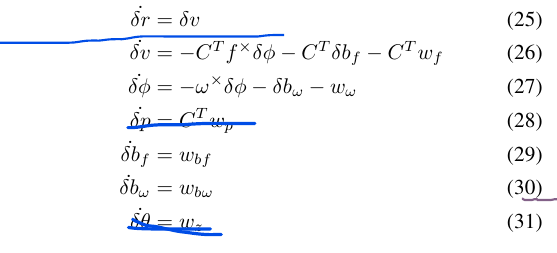
\includegraphics[width=.45\textwidth]{fig03_contModel.png}
        \centering
\end{figure}

\subsection{Discrete Linear Model}
The following depicts what was presented in QEKF2 paper, \cite{rotella2014state}.

\begin{figure}[h]
        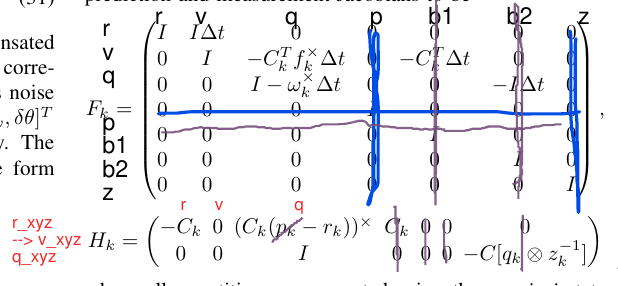
\includegraphics[width=.45\textwidth]{fig02_ldm.png}
        \centering
\end{figure}





\subsection{EKF Update Step}
The following is the standard EKF update step formulation.
\begin{equation}
% \label{eq:}
\begin{split}\begin{array}{rcl}
        {v}_t &=& {z}_t - {h}({x}_t) \\
        {S}_t &=& {H}({x}_t) \hat{{P}}_t {H}^T({x}_t) + {R}_t \\
        {K}_t &=& \hat{{P}}_t {H}^T({x}_t) {S}_t^{-1} \\
        {x}_t &=& \hat{{x}}_t + {K}_t {v}_t \\
        {P}_t &=& \big({I}_4 - {K}_t{H}(x_t)\big)\hat{{P}}_t
\end{array}\end{split}
\end{equation}



\subsection{Update Step Implementation}
The following equations represent our QEKF implementation.
\textcolor{red}{Note: the F and H matrices are not properly implemented?}
\begin{equation}
% \label{eq:}
\begin{split}\begin{array}{lll}
  {H}_{x}  & = & {H}_{12 \times 9} {x}_{k, 9 \times 1}\\
  {S} & = & {H}_{x}\hat{{P}}\transpose{{H}}_{x}+ {R}\\
  {K} & = & \hat{{P}} \transpose{{H}}_{x} {S}^{-1}\\
  {y}_{r,v,w} & = & {z}_{r,v,w} - \transpose{{H}}_{x;r,v,w} \\
  {y}_{q} & = &  \log({z}_{q} \bigotimes   {x}_{q})\\
  {y} & = & \transpose{\left[{y}_{r,v,w}, {y}_{q} \right]}\\
  {x} & = & \hat{{x}} + {K} {y} \\
  {x}_{q} & = & \text{map}_{exp}(\Delta t (Ky_{\omega} )) \\
  P^{+} & = & (I - KH) P^{-} \transpose{(I -KH)} + KR \transpose{K}\\
\end{array}\end{split}
\end{equation}

\noindent
where H is a \(12 \times 9\) matrix. x is a \(9 \times 1\) matrix.




\subsection{Abbreviations and Acronyms}
Defib

\subsection{Units}



\subsection{Equations}

The equations



Note

\subsection{Some Common Mistakes}

\section{USING THE TEMPLATE}

Use this sample docu

\subsection{Headings, etc}

Text heads organiz

\subsection{Figures and Tables}

Positioning Figure



\begin{table}[h]
\caption{An Example of a Table}
\label{table_example}
\begin{center}
\begin{tabular}{|c||c|}
\hline
One & Two\\
\hline
Three & Four\\
\hline
\end{tabular}
\end{center}
\end{table}


   \begin{figure}[thpb]
      \centering
      \framebox{\parbox{3in}{We suggest }}
      %\includegraphics[scale=1.0]{figurefile}
      \caption{Inductance ofd}
      \label{figurelabel}
   \end{figure}




\section{CONCLUSIONS}

A conclu

\addtolength{\textheight}{-12cm}   % This command serves to balance the column lengths
                                  % on the last page of the document manually. It shortens
                                  % the textheight of the last page by a suitable amount.
                                  % This command does not take effect until the next page
                                  % so it should come on the page before the last. Make
                                  % sure that you do not shorten the textheight too much.

%%%%%%%%%%%%%%%%%%%%%%%%%%%%%%%%%%%%%%%%%%%%%%%%%%%%%%%%%%%%%%%%%%%%%%%%%%%%%%%%



%%%%%%%%%%%%%%%%%%%%%%%%%%%%%%%%%%%%%%%%%%%%%%%%%%%%%%%%%%%%%%%%%%%%%%%%%%%%%%%%



%%%%%%%%%%%%%%%%%%%%%%%%%%%%%%%%%%%%%%%%%%%%%%%%%%%%%%%%%%%%%%%%%%%%%%%%%%%%%%%%
\section*{APPENDIX}

Appendixes should appear before the acknowledgment.

\section*{ACKNOWLEDGMENT}

The preferr



%%%%%%%%%%%%%%%%%%%%%%%%%%%%%%%%%%%%%%%%%%%%%%%%%%%%%%%%%%%%%%%%%%%%%%%%%%%%%%%%

\bibliography{ref}
\bibliographystyle{ieeetr}

\end{document}
